\documentclass[11pt,a4paper,slovene]{article}

%Uporabljeni paketi
\usepackage[slovene]{babel}
\usepackage[utf8]{inputenc}
\usepackage{lmodern}
\usepackage[T1]{fontenc}
\usepackage{fancyhdr}
\usepackage{caption}
\captionsetup{font={default,footnotesize}, labelfont=bf, format=hang,indention=.0cm}
\usepackage{graphicx,epsfig}
\usepackage{amsmath}
\usepackage{multirow}
\usepackage{color}
\usepackage{url}
\usepackage{makeidx}
\usepackage[official]{eurosym}
\usepackage{pgfplots}
\usepackage{pgfplotstable}
\usepackage{float}
\pgfplotsset{compat=1.18}

\usepackage{hyperref}
\hypersetup{
   bookmarksnumbered=true,
   urlbordercolor={0 1 0},
   linkbordercolor={1 1 1},
   unicode=true,
   pdftitle={ Ranljivosti Bluetooth naprav },
   pdfauthor={Asistent},
   pdfdisplaydoctitle=true,
   pdftoolbar=true,
   pdfmenubar=true,
   pdfstartview={FitH}
}

\urlstyle{same}

\setlength{\parskip}{12pt}
\setlength\parindent{0pt}
\setlength\unitlength{1mm}

\begin{document}
\label{naslov}
\pdfbookmark[1]{Naslov}{naslov}
\thispagestyle{empty}

\begin{center}
\begin{Large}
Študijsko leto 2024/2025\\
\end{Large}

\vspace*{4cm}
\begin{LARGE}
\textbf{Ranljivosti Bluetooth naprav\\}
\end{LARGE}
\vspace*{0.5cm}

\begin{Large}
Končno poročilo seminarske naloge\\

\vspace*{4cm}

Urban Gajšek\\
Vpisna št. 63220077\\

\vspace*{5cm}
Ljubljana, \today
\end{Large}
\end{center}

\pagebreak
\setcounter{page}{1}
\pagenumbering{arabic}


\label{Kazalo}
\pdfbookmark[1]{Kazalo}{Kazalo}
\tableofcontents
\thispagestyle{empty}
\pagebreak

\section{Uvod}

Bluetooth je brezžična komunikacijska tehnologija za prenos podatkov na kratke razdalje, ki deluje na frekvenčnem območju \texttt{2,4 GHz}. Omogoča povezovanje različnih naprav, kot so pametni telefoni, slušalke, tipkovnice, miške in drugi pametni dodatki, brez potrebe po kablih \cite{networking_A_Z}.

V tej nalogi sem raziskovali varnost in ranljivosti Bluetooth naprav z uporabo različnih orodij, kot so \texttt{hcitool}, \texttt{btmon}, \texttt{l2ping} in \texttt{Wireshark}. Preverjal sem dosegljivost in kakovost povezave z različnimi napravami, meril latenco, generiral dodatni promet in analiziral njegov vpliv na delovanje naprav. Prav tako sem preučil različne vrste napadov na Bluetooth ter metode zaščite pred njimi. Cilj naloge je bil bolje razumeti, kako varna (ali ranljiva) je ta tehnologija in kakšni so najboljši pristopi za njeno zaščito.

\section{Dosegljivost in kakovost povezave}

Da ugotovimo katere naprave so dosegljive, uporabimo ukaz \texttt{hcitool scan}. Ta ukaz skenira okolico in prikaže seznam imen in MAC naslovov Bluetooth naprav, ki jih najde.

Za potrebe te naloge sem uporabljal 4 različne naprave: SilverCrest bluetooh zvočnik (SBL TW6 C2), Sony Bluetooth slušalke (WH-XB910N), Galaxy Buds Pro slušalke in telefon Samsung Galaxy S22 (samo pri preučevanju napadov).

Za merjenje moči povezave sem uporabil program \texttt{btmon}, ki prikazuje podatke o povezavi v realnem času. Za lažje branje podatkov ter shranjevanja in prikazovanja grafov programa nisem zaganjal direktno, temveč sem ga ovil v svoj python program. V svojem programu sem iz izhoda \texttt{btmon} izluščil podatke o moči signala. Podane so bile RSSI vrednosti (Received Signal Strength Indicator) v enotah dBm. Na uradni strani Bluetooh je navedeno, da naj bi RSSI bile relativne vrednosti, ki naj bi bile odvisne od naprave \cite{bluetooth_com}. Iz drugih virov pa sem zasledil, da naj bi bile vrednosti RSSI v dBm in da naj bi bile absolutne, ter da naj bi se gibale od okoli -20dBm (zelo dobra povezava) do -120dBm (naprava komaj zaznana) \cite{bluetoothle_rssi}. V svojih testih sem izmeril vrednosti RSSI v razponu od 0 do -30dBm. Glede na vire sem te vrednosti težko interpretiral kot absolutne vrednosti moči signala, zato sem jih obravnaval kot relativne vrednosti. Vsekakor pa so bile uporabne za določanje vpliva razdalje ter ovir na moč signala.

\subsection{Vpliv razdalje na kakovost povezave}

Vpliv razdalje na moč signala sem izmeril tako, da sem za vsako napravo opravil 3 eksperimente na treh različnih razdaljah (5m, 10m, 15m), nato pa sem še za vsako napravo poiskal razdaljo, na kateri se začne izgubljati povezava. Vsak eksperiment je vseboval 50 meritev iz katerih sem izluščil povprečno vrednost RSSI, nato pa sem povprečil še te tri povprečne vrednosti. Pri meritvah je bila pot od Bluetooth naprave do prenosnega računalnika, na katerega so naprave bile povezane, prosta.

\begin{figure}[H]
\centering
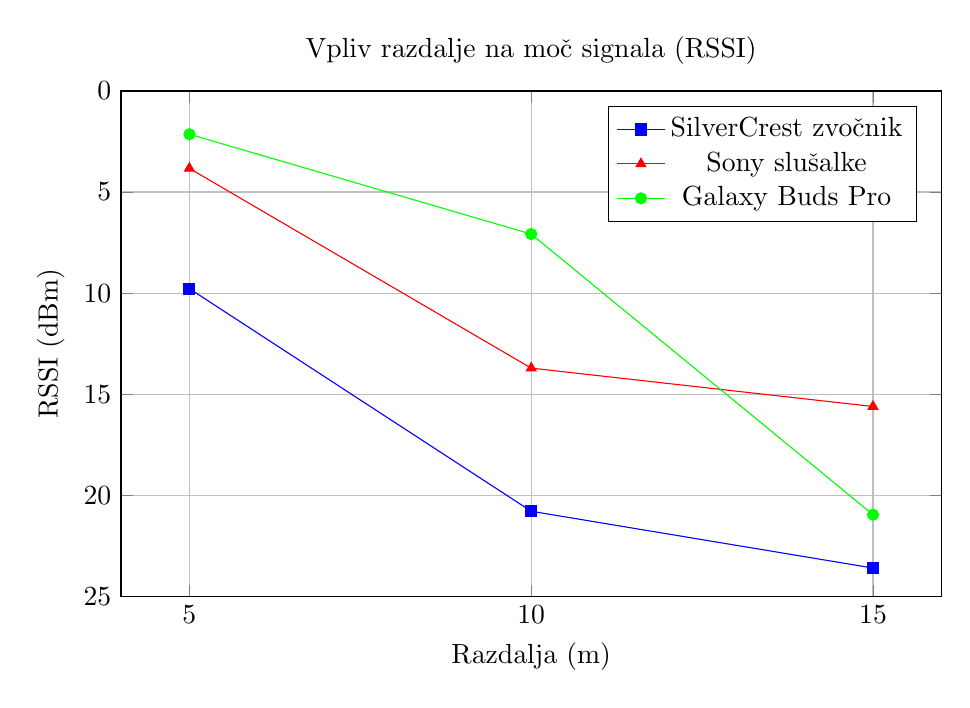
\begin{tikzpicture}
\begin{axis}[
    width=12cm,
    height=8cm,
    title={Vpliv razdalje na moč signala (RSSI)},
    xlabel={Razdalja (m)},
    ylabel={RSSI (dBm)},
    legend pos=north east,
    grid=major,
    y dir=reverse, % ker so nižje vrednosti RSSI slabše
    xtick={5, 10, 15},
    ymin=0, ymax=25
]

\addplot[
    color=blue,
    mark=square*
]
coordinates {
    (5, 9.78)
    (10, 20.79)
    (15, 23.60)
};
\addlegendentry{SilverCrest zvočnik}

\addplot[
    color=red,
    mark=triangle*
]
coordinates {
    (5, 3.83)
    (10, 13.71)
    (15, 15.61)
};
\addlegendentry{Sony slušalke}

\addplot[
    color=green,
    mark=*
]
coordinates {
    (5, 2.14)
    (10, 7.08)
    (15, 20.96)
};
\addlegendentry{Galaxy Buds Pro}

\end{axis}
\end{tikzpicture}
\caption{Meritve moči signala (RSSI) pri različnih razdaljah za tri naprave.}
\label{fig:rssi-graf}
\end{figure}

Kot pričakovano se moč signala z večanjem razdalje zmanjšuje. Med izvajanjem eksperimentov sem opazil, da je moč signala močno nihala. Pri Sony slušalkah sem opazil, da se je moč signala drastično spremenila, samo če sem jih zarotiral za 180 stopinj. Razlog za to je najverjetneje v tem, da je enkrat bila antena obrnjena proti računalniku, drugič pa stran od njega, na svoji poti pa je pri tem signal prepotoval čez celotno ohišje in vezje slušalk \cite{sony_wh_xb910n}.

Zanimalo me je tudi, kako daleč se lahko oddaljim od naprave, da lahko še vedno nemoteno poslušam glasbo. Zaradi konsistentnosti sem na napravah predvajal šum (white noise), zato, da je bil prenos podatkov čim bolj enakomeren. Pri merjenju sem se moral oddaljevati počasi, ter med premikanjem paziti, da ohranim čisto pot do prenosnika. Pri večjih ovinkih ali ovirah se je povezava hitro prekinila.

\begin{figure}[H]
\centering
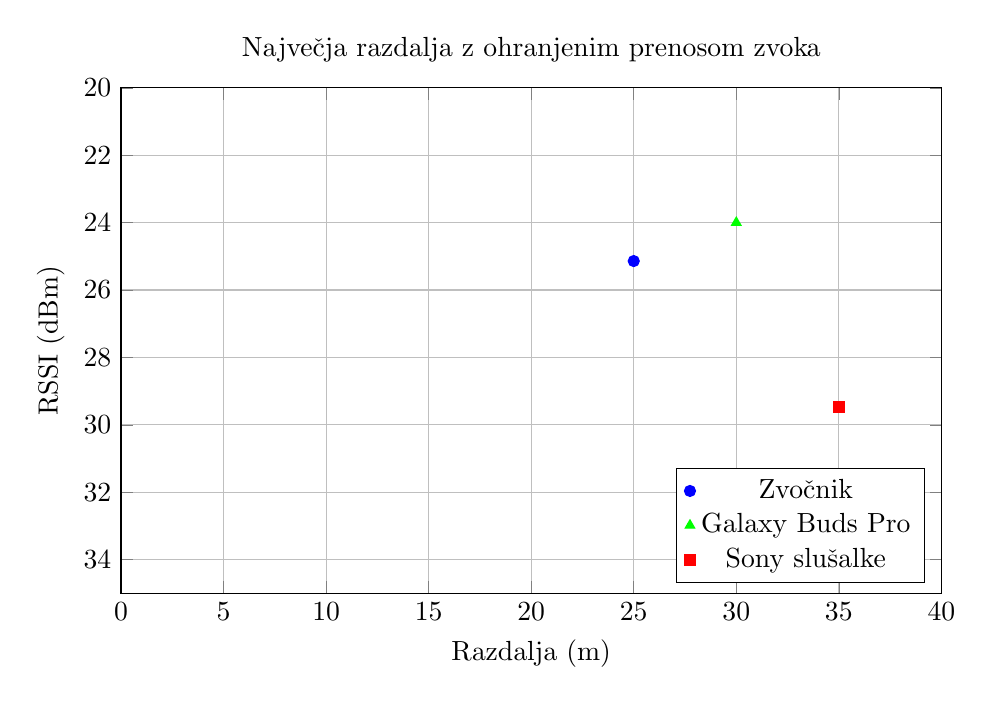
\begin{tikzpicture}
\begin{axis}[
    width=12cm,
    height=8cm,
    title={Največja razdalja z ohranjenim prenosom zvoka},
    xlabel={Razdalja (m)},
    ylabel={RSSI (dBm)},
    y dir=reverse, % manjši dBm = slabši signal
    grid=major,
    xmin=0, xmax=40,
    ymin=20, ymax=35,
    legend style={at={(0.98,0.02)}, anchor=south east}
]

% Naprave
\addplot[
    only marks,
    mark=*,
    color=blue
] coordinates {(25, 25.14)};
\addlegendentry{Zvočnik}

\addplot[
    only marks,
    mark=triangle*,
    color=green
] coordinates {(30, 24.00)};
\addlegendentry{Galaxy Buds Pro}

\addplot[
    only marks,
    mark=square*,
    color=red
] coordinates {(35, 29.48)};
\addlegendentry{Sony slušalke}

\end{axis}
\end{tikzpicture}
\caption{Dosežena največja razdalja za posamezno napravo z nemotenim predvajanjem, ter RSSI na tej razdalji.}
\end{figure}

\subsection{Vpliv ovir na kakovost povezave}

Vpliv ovir na moč signala sem izmeril tako, da sem naprave postavil na določeno razdaljo, za katero imam še izmerjeno povprečno RSSI vrednost, ob prosti poti, nato pa sem na pot postavljal razne ovire.

\begin{figure}[H]
\centering
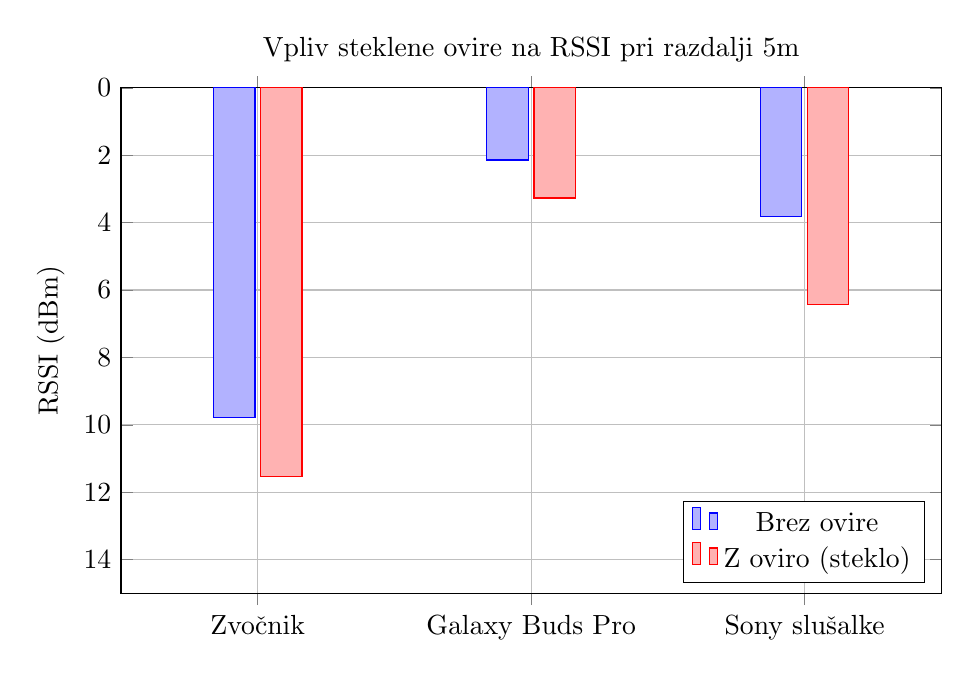
\begin{tikzpicture}
\begin{axis}[
    width=12cm,
    height=8cm,
    ybar,
    bar width=15pt,
    enlarge x limits=0.25,
    symbolic x coords={Zvočnik, Galaxy Buds Pro, Sony slušalke},
    xtick=data,
    ylabel={RSSI (dBm)},
    y dir=reverse, % manjši RSSI pomeni boljši signal
    ymin=0, ymax=15,
    legend style={at={(0.98,0.02)}, anchor=south east},
    grid=major,
    title={Vpliv steklene ovire na RSSI pri razdalji 5m}
]

\addplot+[style={blue,fill=blue!30}] coordinates {
    (Zvočnik, 9.78)
    (Galaxy Buds Pro, 2.14)
    (Sony slušalke, 3.83)
};
\addlegendentry{Brez ovire}

\addplot+[style={red,fill=red!30}] coordinates {
    (Zvočnik, 11.53)
    (Galaxy Buds Pro, 3.27)
    (Sony slušalke, 6.44)
};
\addlegendentry{Z oviro (steklo)}

\end{axis}
\end{tikzpicture}
\caption{Primerjava RSSI vrednosti z in brez 1cm stekla na razdalji 5m}
\end{figure}

\begin{figure}[H]
\centering
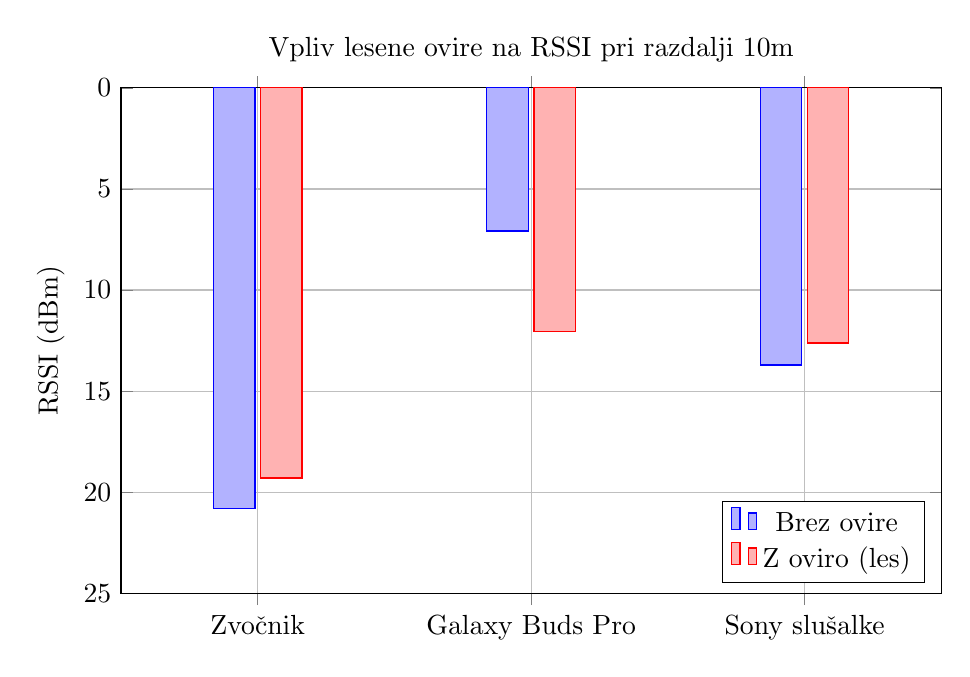
\begin{tikzpicture}
\begin{axis}[
    width=12cm,
    height=8cm,
    ybar,
    bar width=15pt,
    enlarge x limits=0.25,
    symbolic x coords={Zvočnik, Galaxy Buds Pro, Sony slušalke},
    xtick=data,
    ylabel={RSSI (dBm)},
    y dir=reverse, % manjši RSSI pomeni boljši signal
    ymin=0, ymax=25,
    legend style={at={(0.98,0.02)}, anchor=south east},
    grid=major,
    title={Vpliv lesene ovire na RSSI pri razdalji 10m}
]

\addplot+[style={blue,fill=blue!30}] coordinates {
    (Zvočnik, 20.79)
    (Galaxy Buds Pro, 7.08)
    (Sony slušalke, 13.71)
};
\addlegendentry{Brez ovire}

\addplot+[style={red,fill=red!30}] coordinates {
    (Zvočnik, 19.30)
    (Galaxy Buds Pro, 12.03)
    (Sony slušalke, 12.62)
};
\addlegendentry{Z oviro (les)}

\end{axis}
\end{tikzpicture}
\caption{Primerjava RSSI vrednosti z in brez 2cm lesa na razdalji 10m}
\end{figure}

\begin{figure}[H]
\centering
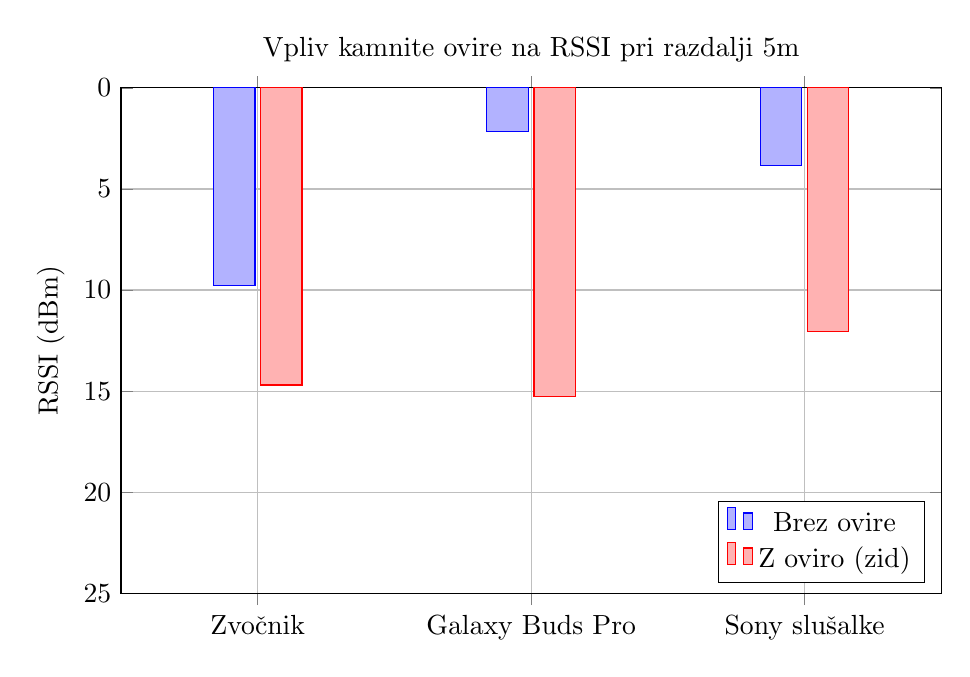
\begin{tikzpicture}
\begin{axis}[
    width=12cm,
    height=8cm,
    ybar,
    bar width=15pt,
    enlarge x limits=0.25,
    symbolic x coords={Zvočnik, Galaxy Buds Pro, Sony slušalke},
    xtick=data,
    ylabel={RSSI (dBm)},
    y dir=reverse, % manjši RSSI pomeni boljši signal
    ymin=0, ymax=25,
    legend style={at={(0.98,0.02)}, anchor=south east},
    grid=major,
    title={Vpliv kamnite ovire na RSSI pri razdalji 5m}
]

\addplot+[style={blue,fill=blue!30}] coordinates {
    (Zvočnik, 9.78)
    (Galaxy Buds Pro, 2.14)
    (Sony slušalke, 3.83)
};
\addlegendentry{Brez ovire}

\addplot+[style={red,fill=red!30}] coordinates {
    (Zvočnik, 14.7)
    (Galaxy Buds Pro, 15.27)
    (Sony slušalke, 12.05)
};
\addlegendentry{Z oviro (zid)}

\end{axis}
\end{tikzpicture}
\caption{Primerjava RSSI vrednosti z in brez 30cm zidu na razdalji 5m}
\end{figure}

Iz grafov je razvidno, da tanke ovire (steklo, les) ne vplivajo močno na moč signala, medtem ko debelejše ovire (zid) povzročijo veliko izgubo moči signala.

\section{Latenca in obremenitve}

Latenco sem meril z ukazom \texttt{l2ping}, ki pošlje paket na napravo in izmeri čas, ki je potreben, da se paket vrne nazaj.

\subsection{Wireshark zajem}
Pri zajemu l2ping paketov z programom Wireshark lahko opazimo, da gre za protokol \texttt{L2CAP} (Logical Link Control and Adaptation Protocol) in da poteka izmenično pošiljanje paketa \texttt{Echo Request} in \texttt{Echo Response}. Vidna je tudi zakasnitev, to pa sem natančneje meril z ukazom \texttt{l2ping}.

\subsection{Latenca ob normalni obremenitvi}

Vse meritve sem opravil na razdalji 30cm brez ovir. Za vsako napravo sem opravil 250 meritev, nato pa izračunal povprečje.

\begin{figure}[H]
\centering
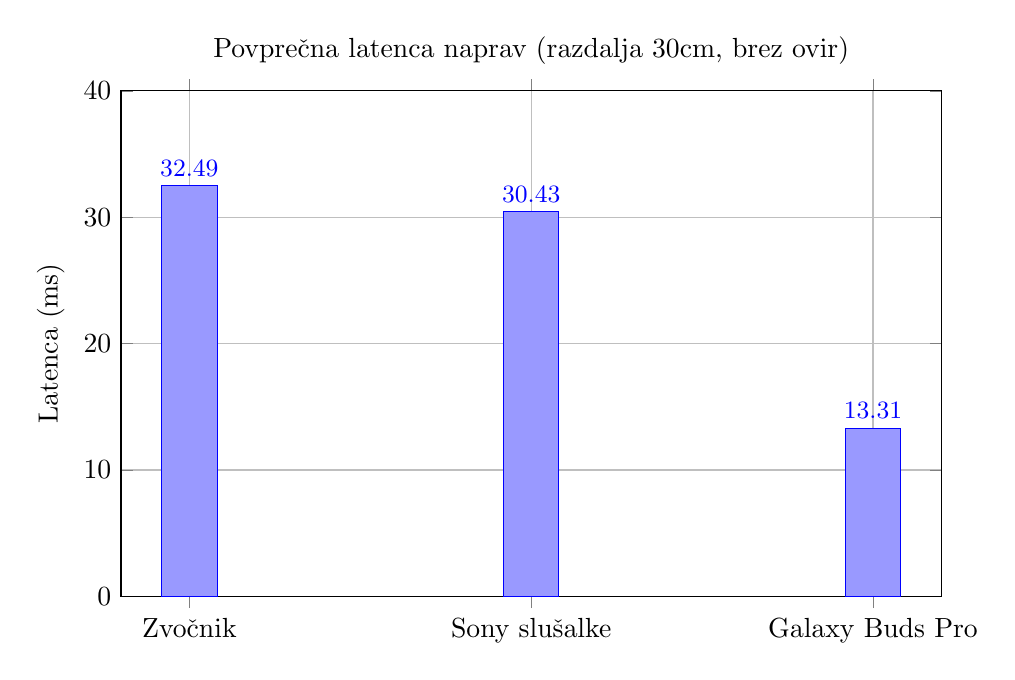
\begin{tikzpicture}
\begin{axis}[
    width=12cm,
    height=8cm,
    ybar,
    bar width=20pt,
    symbolic x coords={Zvočnik, Sony slušalke, Galaxy Buds Pro},
    xtick=data,
    ylabel={Latenca (ms)},
    ymin=0,
    ymax=40,
    grid=major,
    title={Povprečna latenca naprav (razdalja 30cm, brez ovir)},
    nodes near coords,
    every node near coord/.append style={font=\small, anchor=south}
]

\addplot+[style={blue,fill=blue!40}] coordinates {
    (Zvočnik, 32.49)
    (Sony slušalke, 30.43)
    (Galaxy Buds Pro, 13.31)
};

\end{axis}
\end{tikzpicture}
\caption{Povprečna latenca merjena z \texttt{l2ping} (250 paketov)}
\end{figure}

V naslednjem eksperimentu sem želel potrditi, da se latenca povečuje z oddaljenostjo, ne pa tudi z dodatnimi ovirami (dokler ni ovira tako velika, da je povezava tako slaba da se pojalja veliko število napak). Eksperiment sem izvedel samo z zvočnikom.

\begin{figure}[H]
\centering
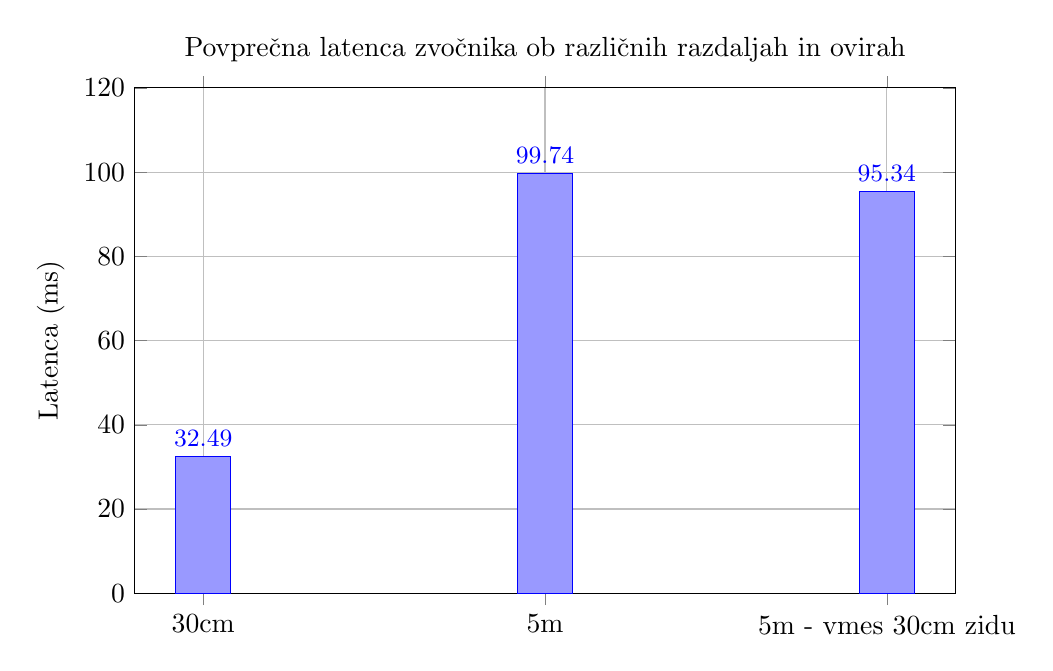
\begin{tikzpicture}
\begin{axis}[
    width=12cm,
    height=8cm,
    ybar,
    bar width=20pt,
    symbolic x coords={30cm, 5m, 5m - vmes 30cm zidu},
    xtick=data,
    ylabel={Latenca (ms)},
    ymin=0,
    ymax=120,
    grid=major,
    title={Povprečna latenca zvočnika ob različnih razdaljah in ovirah},
    nodes near coords,
    every node near coord/.append style={font=\small, anchor=south}
]

\addplot+[style={blue,fill=blue!40}] coordinates {
    (30cm, 32.49)
    (5m, 99.74)
    (5m - vmes 30cm zidu, 95.34)
};

\end{axis}
\end{tikzpicture}
\caption{Povprečna latenca zvočnika merjena z \texttt{l2ping} (250 paketov)}
\end{figure}

Iz grafa je razvidno, da se latenca ni bistveno spremenila z oviro, temveč le z razdaljo.

\subsection{Latenca ob visoki obremenitvi}

V tem eksperimentu sem želel preveriti, kako se latenca spremeni, ko napravo obremenimo z dodatnim prometom. Za to sem uporabil program \texttt{l2ing} in ga pognal z zastavico \texttt{-f} (flood). Zastavica pomeni, da program neprestano pošilja pakete z visoko frekvenco. Paralelno sem poganjal vedno več instanc programa \texttt{l2ping} in meril latenco, dokler se niso začeli izgubljati paketi, oz. dokler se naprava ni izklopila. Ob vsakem številu instanc sem opravil 50 meritev latence in izračunal povprečje.

\begin{figure}[H]
    \centering
    \includegraphics[width=1\textwidth]{images/speaker_stress_latency_25.png}
    \caption{Latenca zvočnika v odvisnosti od števila instanc \texttt{l2ping}}
    \label{fig:speaker_stress_latency}
\end{figure}

\begin{figure}[H]
    \centering
    \includegraphics[width=1\textwidth]{images/buds_stress_latency_80.png}
    \caption{Latenca slušalk Galaxy Buds Pro v odvisnosti od števila instanc \texttt{l2ping}}
    \label{fig:buds_stress_latency}
\end{figure}

\begin{figure}[H]
    \centering
    \includegraphics[width=1\textwidth]{images/sony_stress_latency_80.png}
    \caption{Latenca Sony slušalk v odvisnosti od števila instanc \texttt{l2ping}}
    \label{fig:sony_stress_latency}
\end{figure}

Latenca pričakovano narašča z večanjem števila instanc \texttt{l2ping}. Zvočnik je začel izgubljati pakete že pri 25 procesih, največja latenca pa je znašala kar 800ms. Sony slušalke so se pri 75 instancah celo izklopile.

\section{Napadi na Bluetooth naprave}

Moderne Bluetooth naprave (Bluetooth 6.0, 2024) so večinoma relativno varne. Seveda pa je v obtoku še vedno veliko starejših naprav, prav tako pa je še vedno obstajajo ranljivosti, ki jih je mogoče izkoristiti tudi na novejših napravah.

\subsection{Pregled pogostih napadov}
\begin{itemize}
    \item \textbf{MAC Address tracking} - Ko je naprava v načinu iskanja, je njen MAC naslov viden vsem napravam v bližini. To samo po sebi ni ranjljivost, vendar je velikokrat prvi korak v mnogih drugih napadih. Ker se MAC naslov naprave načeloma ne spreminja (nekatere moderne naprave ga lahko naključno spremenijo), ga lahko uporabimo kot identifikator naprave in posledično uporabnika. Trgovine bi to lahko uporabile za sledenje uporabnikom in preučevanje vzorcev nakupovalnih časov.
    \item \textbf{Bluejacking} - Napravi pošljemo sporočilo brez dovoljenja uporabnika. Največkrat posledice niso resne, uporabniku se lahko na primer prikaže oglasno sporočilo. Večina modernih naprav takih sporočil ne sprejema več, oz. zahtevajo, da jih uporabnik eksplicitno sprejme.
    \item \textbf{Bluesnarfing} - Iz naprave pridobimo zasebne podatke, kot so stiki, koledarji, sporočila in podobno. Večina modernih naprav zahteva, da uporabnik izrecno dovoli dostop do teh podatkov. 
    \item \textbf{Bluebugging} - Pridobimo popoln nadzor nad napravo. Na modernih napravah je to brez posebnih nastavitev skoraj nemogoče.
    \item \textbf{Bluetooth spoofing} - MAC naslov lastne naprave spremenimo v MAC naslov druge naprave in jo s tem impersoniramo. To je lahko uporabno pri naslednjem napadu.
    \item \textbf{MITM} - Prestrežemo komunikacijo med dvema napravama. Povezati se moramo z obema napravama, nato pa se podatki prenašajo preko nas, mi pa jih posredujemo naprej.
    \item \textbf{DoS napadi} - Napravo preobremenimo z mnogo paketi, poslanimi z visoko frekvenco. Naprava se lahko izklopi ali začne počasneje delovati in izgubljati pakete. V skrajnih primerih se lahko naprava celo pregreje in uniči. Primer tega je uporaba zastavice \texttt{-f} pri ukazu \texttt{l2ping}, ki pošilja pakete z visoko frekvenco.
\end{itemize}

\subsection{Demonstracija izvedljivih napadov}

Najprejprej preglejmo dosegljive Bluetooth naprave:
\begin{verbatim}
$ hcitool scan
Scanning ...
        41:42:7B:CB:AC:9E       SBL TW6 C2
        44:EA:30:60:EA:58       Galaxy Buds Pro (EA58)
        F0:CD:31:60:0F:D5       Urban S22
        90:7A:58:E9:9A:BB       WH-XB910N
\end{verbatim}

Zgoraj vidimo 4 prej omenjene naprave in njihove MAC naslove. Demonstracijo bom nadaljeval na telefonu S22, zato si bom za lažje delo shranil njegov MAC naslov:

\begin{verbatim}
$ PHONE_MAC=F0:CD:31:60:0F:D5
\end{verbatim}

Sedaj ko imam shranjen MAC naslov, lahko poiskušam ugotoviti, kakše storitve naprava podpira. To lahko storimo s pomočjo \texttt{sdptool}:
\begin{verbatim}
$ sdptool browse $PHONE_MAC
...
Service Name: OBEX Object Push
Service RecHandle: 0x10053
Service Class ID List:
  "OBEX Object Push" (0x1105)
Protocol Descriptor List:
  "L2CAP" (0x0100)
  "RFCOMM" (0x0003)
    Channel: 12
  "OBEX" (0x0008)
Profile Descriptor List:
  "OBEX Object Push" (0x1105)
    Version: 0x0102
...
\end{verbatim}

Med drugim je \texttt{sdptool} našel tudi storitev \texttt{OBEX Object Push}, ki omogoča pošiljanje datotek na napravo. To storitev lahko preiskusimo:

\begin{verbatim}
$ obexftp --noconn --uuid none --bluetooth $PHONE_MAC --channel 12 --put test.txt

Suppressing FBS.
Connecting..\done
Sending "test.txt".../done
Disconnecting..-done    
\end{verbatim}

S tem ukazom sem uspešno poslal datoteko \texttt{test.txt} na svoj telefon, brez da bi prej vzpostavil Bluetooth povezavo. Na telefonu sem sicer še vedno moral eksplicitno potrditi prejem datoteke, vendar pa se vsekakor lahko zgodi napaka nepozornega uporabnika, ki potrdi prejem datoteke, ki je ne želi.

Relativno enostavna je tudi izvedba \texttt{l2ping flood} napada. V tem primeru sem uporabil \texttt{l2ping} z zastavico \texttt{-f}:

\begin{verbatim}
$ sudo l2ping -s 600 -f $PHONE_MAC
Ping: F0:CD:31:60:0F:D5 from 64:79:F0:53:DD:37 (data size 600) ...
600 bytes from F0:CD:31:60:0F:D5 id 0 time 27.76ms
600 bytes from F0:CD:31:60:0F:D5 id 1 time 40.01ms
600 bytes from F0:CD:31:60:0F:D5 id 2 time 36.01ms
600 bytes from F0:CD:31:60:0F:D5 id 3 time 67.96ms
600 bytes from F0:CD:31:60:0F:D5 id 4 time 23.93ms
600 bytes from F0:CD:31:60:0F:D5 id 5 time 31.90ms
600 bytes from F0:CD:31:60:0F:D5 id 6 time 48.26ms
600 bytes from F0:CD:31:60:0F:D5 id 7 time 35.96ms
600 bytes from F0:CD:31:60:0F:D5 id 8 time 24.10ms
600 bytes from F0:CD:31:60:0F:D5 id 9 time 23.79ms
600 bytes from F0:CD:31:60:0F:D5 id 10 time 27.85ms
600 bytes from F0:CD:31:60:0F:D5 id 11 time 40.14ms
600 bytes from F0:CD:31:60:0F:D5 id 12 time 27.88ms
600 bytes from F0:CD:31:60:0F:D5 id 13 time 24.10ms
...
\end{verbatim}

Ta ukaz sam po sebi modernim napravem ne povzroči vidnih sprememb, če pa poženemo več instanc \texttt{l2ping} pa lahko naprava začne izgubljati pakete, ali pa se celo izklopi.

\section{Možni pristopi zaščite}

Sodobne naprave imajo večinoma varne nastavitve, še vedno pa se je dobro zavedati potencialnih ranljivosti in se jim izogniti.

\begin{itemize}
    \item \textbf{Onemogočite Bluetooth} - Najboljši način zaščite je, da Bluetooth izklopite, ko ga ne potrebujete. Kadar je Bluetooth izklopljen, naprava ne more biti napadena.
    \item \textbf{Onemogočite iskanje} - Ko naprava ni v načinu iskanja, je njen MAC naslov skrit pred drugimi napravami. Tako se izognete napadom, ki zahtevajo iskanje. Večina modernih naprav ob samem vklopu še ne preidejo v stanje iskanja, temveč je potrebna posebna akcija uporabnika.
    \item \textbf{Redno posodabljajte naprave} - Posodobitve vsebujejo popravke ranljivosti in izboljšave varnosti. Ko je odrita nova ranljuvost, se jo lahko s posodobitvijo programske opreme odpravi.
    \item \textbf{Brisanje neuporabljenih/neznanih naprav} - Naprave, ki jih ne uporabljate več, izbrišite iz seznama povezanih naprav. Veliko naprav, ki so na seznamu imajo možnost samodejne vspostavitve povezave ob vklopu Bluetootha.
    \item \textbf{Zavračanje sumljivih potrjevanj} - Vedno potrdimo samo zahteve ali povezave, ki smo jih sami sprožili, oz. za katere smo prepričani, da so varne.
\end{itemize}

\section{Zaključek}

Pri meritvah moči signala sem potrdil precej samoumevne hipoteze o vplivu razdalje na moč signala. Presenetilo me je recimo to, da so bile meritve zelo občutljive, zato sem jih moral izvesti več. Pričakoval sem tudi večji vpliv lesenih vrat na moč signala, vendar pa se je izkazalo, da je bil vpliv neopazen. Pri merjenju latence sem potrdil, da se latenca povečuje z večanjem razdalje, ne pa tudi z dodatnimi ovirami. Pri napadih me je presenetilo to, da se še vedno z lahkoto izvede \texttt{l2ping flood} napad, ki je v primeru Sony slušalk celo povzročil izklop naprave. Čeprav se varnost Bluetooth naprav veča je še vedno potrebna previdnost.

\pagebreak
\bibliographystyle{plain}
\bibliography{references}

\end{document}
